% Provenance (never printed): see sources/outline_sources.md and sources/book1/BRIEFS.md (g4/01).
\chapter{Memory and Storage}\label{ch:g4:memory-and-storage}

Mia has been playing a game for an hour. She has crossed three rivers and
opened two castles. Suddenly the lights go out: the power is cut in the whole
street. When it comes back and she starts the game again, she is back at the
first river, where the game last saved her progress. The \omterm{def:g1:what-is-a-computer:computer}{computer} forgot
everything since then. Why does a \omterm{def:g1:what-is-a-computer:computer}{computer} forget some things and keep others?

\begin{recall}
The \omterm{def:g3:inside-the-computer:processor}{processor} carries out the \omterm{def:g1:instructions-in-order:instruction}{instructions}; the \omterm{def:g3:inside-the-computer:memory}{memory} holds the work in
progress and forgets it when the power goes off; the \omterm{def:g3:inside-the-computer:storage}{storage} keeps the saved
work (\cref{ch:g3:inside-the-computer}).
\end{recall}

\section{RAM: fast, and emptied when the power goes}

\begin{definition}[RAM]\label{def:g4:memory-and-storage:ram}
\emph{RAM}\index{RAM} (random-access \omterm{def:g3:inside-the-computer:memory}{memory}) is the \omterm{def:g3:inside-the-computer:memory}{memory} of a \omterm{def:g1:what-is-a-computer:computer}{computer}: chips on small boards
that hold the information the \omterm{def:g3:inside-the-computer:processor}{processor} is working on. The \omterm{def:g3:inside-the-computer:processor}{processor} can read
and change any part of it very fast, in any order (this is what ``random access'' means), but everything in it is lost when the
power goes off.
\end{definition}

\omterm{def:g4:memory-and-storage:ram}{RAM} keeps information as tiny electric charges, which must be refreshed many
times a second. When the electricity stops, the charges leak away within a
moment, and the \omterm{def:g4:memory-and-storage:ram}{RAM} is empty. That is what happened to Mia's game: her progress
since the last save was only in the \omterm{def:g4:memory-and-storage:ram}{RAM}.

\begin{omfigure}
\begin{tikzpicture}[x=1cm, y=1cm, font=\footnotesize,
    box/.style={draw=black!60, rounded corners=2pt, minimum width=2.6cm, minimum height=1.1cm, align=center}]
  \node[font=\small\bfseries] at (2.0,2.3) {power on};
  \node[box, fill=ocBlue!20] at (0.6,1.0) {RAM\\{\scriptsize game now:}\\{\scriptsize third river}};
  \node[box, fill=ocMint!25] at (3.4,1.0) {SSD\\{\scriptsize last save:}\\{\scriptsize first river}};
  \draw[black!30] (5.2,-0.2) -- (5.2,2.5);
  \node[font=\small\bfseries] at (8.4,2.3) {power off, then on again};
  \node[box, fill=black!5, text=black!50] at (7.0,1.0) {RAM\\{\scriptsize empty}\\{\scriptsize\phantom{x}}};
  \node[box, fill=ocMint!25] at (9.8,1.0) {SSD\\{\scriptsize last save:}\\{\scriptsize first river}};
\end{tikzpicture}

{\small What Mia's \omterm{def:g1:what-is-a-computer:computer}{computer} holds before and after the power cut. Only what
was saved to the \omterm{def:g3:inside-the-computer:storage}{storage} is still there.}
\label{fig:g4:memory-and-storage:power}
\end{omfigure}

\section{Storage that keeps everything}

A \omterm{def:g1:what-is-a-computer:computer}{computer} also needs a place where information stays without electricity.
There are two main kinds.

\begin{definition}[Hard disk]\label{def:g4:memory-and-storage:hard-disk}
A \emph{hard disk}\index{hard disk} stores information on spinning metal
disks covered with a thin magnetic layer. A read--write head, at the end of a
moving arm, flies just above the surface: it writes by making tiny areas
magnetic in one direction or the other, and reads them back.
\end{definition}

The head never touches the disk: it floats on a cushion of air thinner than a
hair. The disks turn thousands of times a minute, so a \omterm{def:g4:memory-and-storage:hard-disk}{hard disk} hums and gets
warm, and a hard knock while it is running can make the head scratch the disk.

\begin{omfigure}
\begin{tikzpicture}[x=1cm, y=1cm, font=\footnotesize, lab/.style={font=\footnotesize, anchor=west}]
  % top view
  \draw[black!70, fill=black!10, rounded corners=4pt] (0,0) rectangle (5.4,6.2);
  \draw[black!60, fill=black!3] (2.4,3.6) circle (2.2);
  \draw[black!25] (2.4,3.6) circle (1.6) (2.4,3.6) circle (1.0);
  \draw[black!70, fill=black!35] (2.4,3.6) circle (0.38);
  \draw[-{Stealth[length=2mm]}, ocBlue!80!black, thick] (2.4,3.6) ++(50:1.9) arc[start angle=50, end angle=95, radius=1.9];
  % arm
  \draw[black!70, fill=black!30] (4.5,0.9) circle (0.35);
  \draw[black!70, fill=black!20] (4.3,1.1) -- (3.15,3.15) -- (3.35,3.3) -- (4.75,1.25) -- cycle;
  \fill[ocRed!80!black] (3.25,3.22) circle (0.09);
  % motor coil
  \draw[black!60, fill=ocYellow!40] (4.65,0.4) rectangle (5.2,1.0);
  % labels
  \draw[black!60] (1.0,5.2) -- (6.0,5.8) node[lab] {disk (platter), spinning};
  \draw[black!60] (2.4,3.6) -- (6.0,4.7) node[lab] {spindle and motor};
  \draw[black!60] (3.25,3.22) -- (6.0,3.4) node[lab] {read--write head};
  \draw[black!60] (3.9,2.0) -- (6.0,2.2) node[lab] {arm};
  \draw[black!60] (4.9,0.7) -- (6.0,0.9) node[lab] {pivot: the arm swings};
  % side view
  \begin{scope}[shift={(0,-1.3)}]
    \fill[black!3] (0,0) rectangle (5.4,0.35);
    \draw[black!70] (0,0.35) -- (5.4,0.35) (0,0) -- (5.4,0);
    \fill[ocBlue!25] (0,0.35) rectangle (5.4,0.42);
    \draw[black!70, fill=black!20] (2.0,0.62) -- (5.4,0.9) -- (5.4,1.05) -- (2.0,0.75) -- cycle;
    \draw[black!70, fill=ocRed!70] (1.8,0.55) rectangle (2.2,0.75);
    \draw[{Stealth[length=1.5mm]}-{Stealth[length=1.5mm]}, black!70] (2.6,0.42) -- (2.6,0.67);
    \node[lab] at (6.0,0.55) {side view: the head flies just above};
    \node[lab] at (6.0,0.15) {the magnetic layer and never touches it};
  \end{scope}
\end{tikzpicture}

{\small A \omterm{def:g4:memory-and-storage:hard-disk}{hard disk} seen from above, and the head seen from the side (the gap
is drawn far larger than it is).}
\label{fig:g4:memory-and-storage:hdd}
\end{omfigure}

\begin{omfigure}
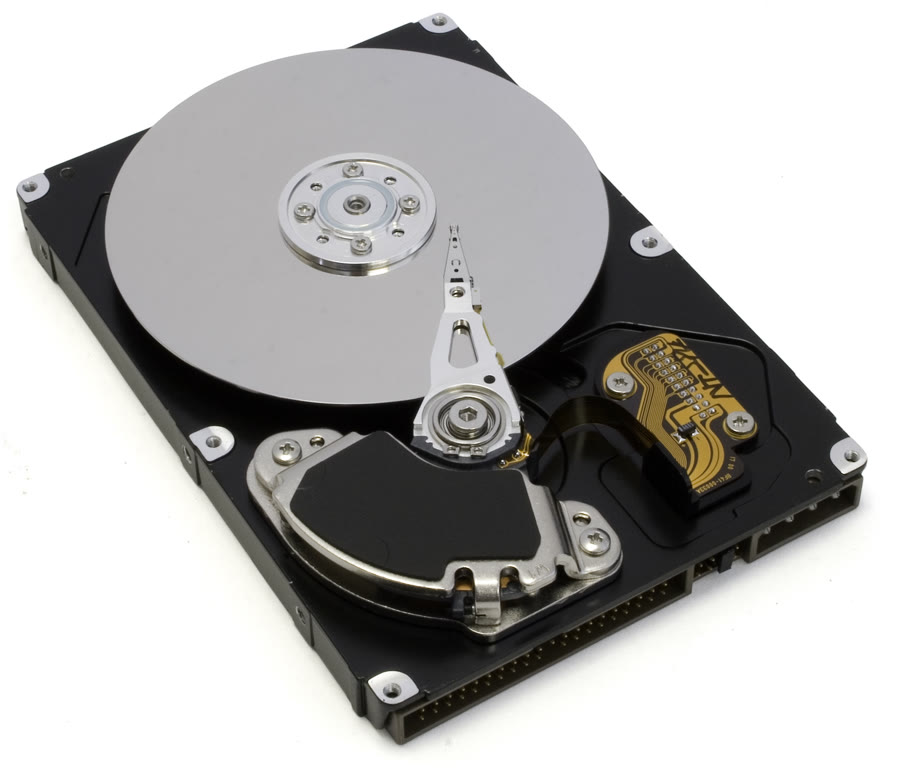
\includegraphics[width=0.45\linewidth]{images/book1/g4-open-hard-disk.jpg}

{\small A real \omterm{def:g4:memory-and-storage:hard-disk}{hard disk} with its lid removed: the shiny disk, the arm with
the head at its tip, and the pivot at the bottom. Photograph: Zzubnik, public
domain.}
\end{omfigure}

\begin{definition}[Flash memory and SSD]\label{def:g4:memory-and-storage:flash}
\emph{Flash memory}\index{flash memory} keeps information as electric
charges trapped in tiny cells of a chip, so tightly that they stay without
electricity for years. An \emph{SSD}\index{SSD} (solid-state drive) is a
\omterm{def:g3:inside-the-computer:storage}{storage} made of flash \omterm{def:g3:inside-the-computer:memory}{memory} chips, with no moving part.
\end{definition}

USB sticks and the \omterm{def:g3:inside-the-computer:memory}{memory} cards of cameras and phones are made of \omterm{def:g4:memory-and-storage:flash}{flash memory}
too. Phones, tablets and most new laptops have an \omterm{def:g4:memory-and-storage:flash}{SSD} instead of a \omterm{def:g4:memory-and-storage:hard-disk}{hard disk}.

\begin{center}
\begin{tabular}{lll}
\hline
 & \omterm{def:g4:memory-and-storage:hard-disk}{hard disk} & \omterm{def:g4:memory-and-storage:flash}{SSD}, USB stick, \omterm{def:g3:inside-the-computer:memory}{memory} card \\
\hline
how it keeps information & magnetic layer on spinning disks & charges trapped in chips \\
moving parts & yes: disks and an arm & none \\
speed & slower: the head must move & faster \\
noise & a soft hum & silent \\
if dropped while running & the disk can be scratched & usually no harm \\
\hline
\end{tabular}
\end{center}

\section{Measuring size in bytes}

How much work can a \omterm{def:g3:inside-the-computer:storage}{storage} hold? We count it in \omterm{def:g4:memory-and-storage:byte}{bytes}.

\begin{definition}[Byte]\label{def:g4:memory-and-storage:byte}
The \emph{byte}\index{byte} is the unit used to measure the size of
information in a \omterm{def:g1:what-is-a-computer:computer}{computer}: one byte holds one letter of plain text.
\end{definition}

% ledger: g4:si-prefixes
\begin{definition}[Kilobyte, megabyte, gigabyte, terabyte]\label{def:g4:memory-and-storage:units}
A \emph{kilobyte}\index{kilobyte} (kB) is \num{1000} \omterm{def:g4:memory-and-storage:byte}{bytes}. A
\emph{megabyte}\index{megabyte} (MB) is \num{1000} kilobytes. A
\emph{gigabyte}\index{gigabyte} (GB) is \num{1000} megabytes. A
\emph{terabyte}\index{terabyte} (TB) is \num{1000} gigabytes.
\end{definition}

Each unit is a thousand times the one before, as a kilometre is a thousand
metres. Let us compute a few sizes.

\begin{example}[A page, a photo, a film]\label{ex:g4:memory-and-storage:sizes}
\begin{itemize}
\item A page of a story has about \num{2000} letters and spaces: about
  \num{2000} \omterm{def:g4:memory-and-storage:byte}{bytes}, so about 2 \omterm{def:g4:memory-and-storage:units}{kilobytes}.
\item A photo of \num{1000} by \num{1000} coloured dots has
  \num{1000000} dots. If each dot is kept as 3 \omterm{def:g4:memory-and-storage:byte}{bytes} (one for each of three
  colours), the photo takes \num{3000000} \omterm{def:g4:memory-and-storage:byte}{bytes}: 3 \omterm{def:g4:memory-and-storage:units}{megabytes}.
\item A film shows 25 pictures every second. If each picture were kept like
  that photo, one second would take $25 \times 3 = 75$ \omterm{def:g4:memory-and-storage:units}{megabytes}, and one
  minute $60 \times 75 = \num{4500}$ \omterm{def:g4:memory-and-storage:units}{megabytes}: 4.5 \omterm{def:g4:memory-and-storage:units}{gigabytes}. Real films are
  packed much more tightly; how this works comes in a later year.
\end{itemize}
\end{example}

\begin{omfigure}
\begin{tikzpicture}[x=1cm, y=1cm, font=\footnotesize,
    sizestep/.style={draw=black!60, fill=ocBlue!12, rounded corners=2pt, minimum width=2.4cm, minimum height=0.7cm, font=\small\bfseries},
    ex/.style={font=\footnotesize, anchor=west, align=left}]
  \foreach \u/\k in {1 byte/0, 1 kilobyte/1, 1 megabyte/2, 1 gigabyte/3, 1 terabyte/4} {
    \node[sizestep] (s\k) at (1.6*\k, 1.15*\k) {\u};
  }
  \foreach \a/\b in {0/1, 1/2, 2/3, 3/4} {
    \draw[-{Stealth[length=2mm]}, black!60] (s\a.north) |- node[pos=0.25, left, font=\scriptsize] {$\times\,\num{1000}$} (s\b.west);
  }
  \node[ex] at (1.6*0+1.4, 1.15*0) {one letter};
  \node[ex] at (1.6*1+1.4, 1.15*1) {a page of a story: 2 kB};
  \node[ex] at (1.6*2+1.4, 1.15*2) {a photo: 3 MB};
  \node[ex] at (1.6*3+1.4, 1.15*3) {one minute of film, unpacked: 4.5 GB};
  \node[ex] at (1.6*4+1.4, 1.15*4) {two million books of 250 pages};
\end{tikzpicture}

{\small The ladder of sizes, from one letter to a \omterm{def:g4:memory-and-storage:units}{terabyte}. Each step is a
thousand times the one below. A book of 250 pages of 2 \omterm{def:g4:memory-and-storage:units}{kilobytes} takes 500
\omterm{def:g4:memory-and-storage:units}{kilobytes}, so a \omterm{def:g4:memory-and-storage:units}{terabyte} holds two million such books.}
\label{fig:g4:memory-and-storage:ladder}
\end{omfigure}

% ledger: g4:iec-binary-prefixes
\begin{remark}[\num{1024} instead of \num{1000}]\label{rem:g4:memory-and-storage:1024}
Some programs count a \omterm{def:g4:memory-and-storage:units}{kilobyte} as \num{1024} \omterm{def:g4:memory-and-storage:byte}{bytes} instead of \num{1000},
for reasons we meet in a later year. The difference is small, but it is why a
\omterm{def:g3:inside-the-computer:storage}{storage} sold as 500 \omterm{def:g4:memory-and-storage:units}{gigabytes} may be shown by the \omterm{def:g1:what-is-a-computer:computer}{computer} as a little less.
The careful name for \num{1024} \omterm{def:g4:memory-and-storage:byte}{bytes} is a kibibyte (KiB).
\end{remark}

\begin{history}[Five million letters on fifty disks]
% ledger: g4:ibm350-date, g4:ibm350-disks, g4:ibm350-capacity, g4:ibm350-size
The first \omterm{def:g4:memory-and-storage:hard-disk}{hard disk} sold for a \omterm{def:g1:what-is-a-computer:computer}{computer} was shipped in June 1956. It was a
cabinet about \qty{1.5}{\metre} high and \qty{1.8}{\metre} wide that weighed,
with its air pump, more than a tonne. Inside, 50 metal disks, each about
\qty{61}{\centi\metre} across, turned \num{1200} times a minute. All together
they held five million letters: less than 4 \omterm{def:g4:memory-and-storage:units}{megabytes}, the size of a single
photo today.
\end{history}

\begin{omfigure}
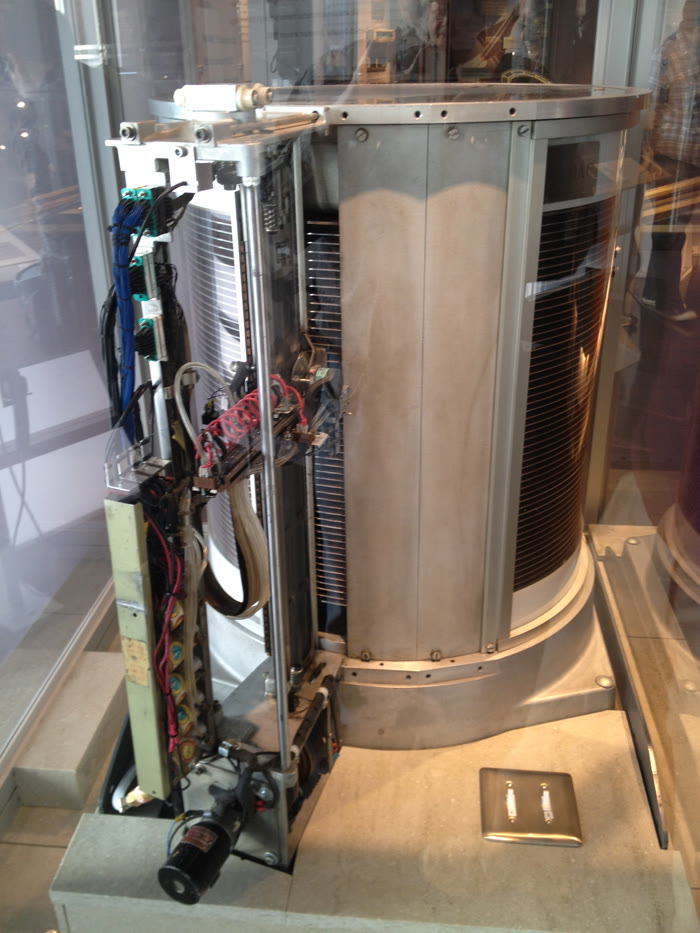
\includegraphics[width=0.36\linewidth]{images/book1/g4-ibm350.jpg}

{\small The stack of disks of a 1956 \omterm{def:g4:memory-and-storage:hard-disk}{hard disk}, in a museum. Photograph:
Arnold Reinhold, CC BY-SA 3.0.}
\end{omfigure}

\section{Why keep a backup}

\omterm{def:g3:inside-the-computer:storage}{Storage} keeps work when the power is off, but it is not safe forever. A \omterm{def:g4:memory-and-storage:hard-disk}{hard
disk} can wear out, a laptop can be dropped, lost or stolen, a \omterm{def:g3:files-and-folders:file}{file} can be
deleted by mistake.

\begin{definition}[Backup]\label{def:g4:memory-and-storage:backup}
A \emph{backup}\index{backup} is a second copy of \omterm{def:g3:files-and-folders:file}{files}, kept on another
\omterm{def:g3:inside-the-computer:storage}{storage}, in another place, so that they can be brought back if the first copy
is lost.
\end{definition}

\begin{omfigure}
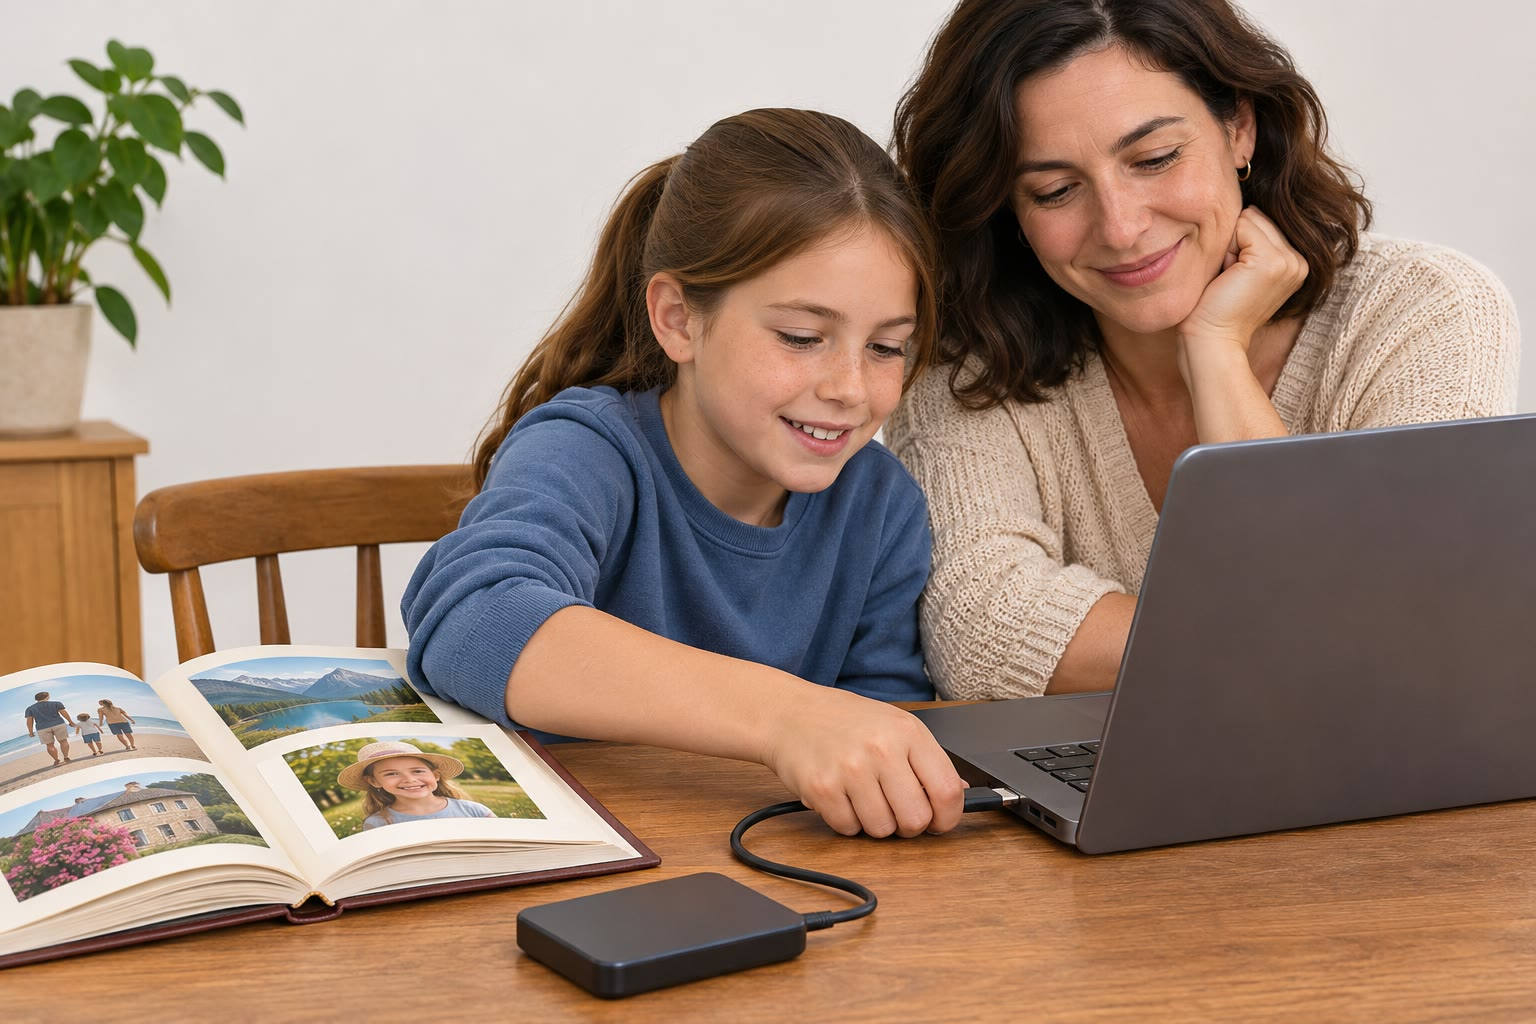
\includegraphics[width=0.5\linewidth]{images/book1/ai/g4-memory-and-storage-backup.jpg}

{\small Backing up the family photos on an external disk.}
\end{omfigure}


\begin{safety}
Keep a \omterm{def:g4:memory-and-storage:backup}{backup} of the work you care about, on another \omterm{def:g3:inside-the-computer:device}{device} and in another
place (a disk kept at home for a school laptop, for example). Update it
often: a \omterm{def:g4:memory-and-storage:backup}{backup} only holds what was there on the day it was made.
\end{safety}

\section{Exercises}

\begin{exercise}[$\star$]\label{exo:g4:memory-and-storage:1}
The power goes off. Which keeps the work: the \omterm{def:g4:memory-and-storage:ram}{RAM} or the \omterm{def:g4:memory-and-storage:flash}{SSD}?
\end{exercise}

\begin{exercise}[$\star$]\label{exo:g4:memory-and-storage:2}
Give two differences between a \omterm{def:g4:memory-and-storage:hard-disk}{hard disk} and an \omterm{def:g4:memory-and-storage:flash}{SSD}.
\end{exercise}

\begin{exercise}[$\star$]\label{exo:g4:memory-and-storage:3}
How many \omterm{def:g4:memory-and-storage:units}{kilobytes} are there in 3 \omterm{def:g4:memory-and-storage:units}{megabytes}?
\end{exercise}

\begin{exercise}[$\star$]\label{exo:g4:memory-and-storage:4}
A page of text takes 2 \omterm{def:g4:memory-and-storage:units}{kilobytes}. How many such pages fit in 1 \omterm{def:g4:memory-and-storage:units}{megabyte}?
\end{exercise}

\begin{exercise}[$\star$]\label{exo:g4:memory-and-storage:5}
Put these sizes in order, from the smallest to the largest: 3 GB, 500 kB,
2 TB, 40 MB, 900 \omterm{def:g4:memory-and-storage:byte}{bytes}.
\end{exercise}

\begin{exercise}[$\star$]\label{exo:g4:memory-and-storage:6}
Why should a \omterm{def:g4:memory-and-storage:backup}{backup} be kept in another place than the \omterm{def:g1:what-is-a-computer:computer}{computer} it copies?
\end{exercise}

\begin{exercise}[$\star$]\label{exo:g4:memory-and-storage:7}
Read the ladder of sizes: how big is one photo? About how many such photos
fit in 1 \omterm{def:g4:memory-and-storage:units}{gigabyte}?
\end{exercise}

\begin{exercise}[$\star$]\label{exo:g4:memory-and-storage:8}
A USB stick holds 64 \omterm{def:g4:memory-and-storage:units}{gigabytes}. Each photo takes 4 \omterm{def:g4:memory-and-storage:units}{megabytes}. How many photos
fit on the stick?
\end{exercise}

\begin{exercise}[$\star\star$]\label{exo:g4:memory-and-storage:9}
A story has \num{12000} letters and spaces. How many \omterm{def:g4:memory-and-storage:units}{kilobytes} does it take?
\end{exercise}

\begin{exercise}[$\star\star$]\label{exo:g4:memory-and-storage:10}
In the story at the start of this chapter, which part of the \omterm{def:g1:what-is-a-computer:computer}{computer} forgot
Mia's progress? Where was the progress she found again?
\end{exercise}

\begin{exercise}[$\star\star$]\label{exo:g4:memory-and-storage:11}
The class keeps all its work on one school \omterm{def:g1:what-is-a-computer:computer}{computer}. Make a plan of \omterm{def:g4:memory-and-storage:backup}{backups}:
on what, where, and how often.
\end{exercise}
